\documentclass{article}%
\usepackage[T1]{fontenc}%
\usepackage[utf8]{inputenc}%
\usepackage{lmodern}%
\usepackage{textcomp}%
\usepackage{lastpage}%
\usepackage[head=40pt,margin=0.5in,bottom=0.6in]{geometry}%
\usepackage{graphicx}%
%
\title{\textbf{Los habitantes del último reducto de ISIS en Siria siguen saliendo}}%
\author{AFP}%
\date{07/03/2019}%
%
\begin{document}%
\normalsize%
\maketitle%
\textbf{URL: }%
http://www.eluniversal.com/internacional/34908/los{-}habitantes{-}del{-}ultimo{-}reducto{-}de{-}isis{-}en{-}siria{-}siguen{-}saliendo\newline%
%
\textbf{Periodico: }%
EU, %
ID: %
34908, %
Seccion: %
internacional\newline%
%
\textbf{Palabras Claves: }%
NO\_TIENE\newline%
%
\textbf{Derecho: }%
2.1%
, Otros Derechos: %
\newline%
%
\textbf{\textit{Los combatientes árabo{-}kurdos de las Fuerzas Democráticas Sirias habían reanudado el viernes su ofensiva en la localidad de Baghuz, pero tuvieron que interrumpirla ya que miles de mujeres y niños}}%
\newline%
\newline%
%
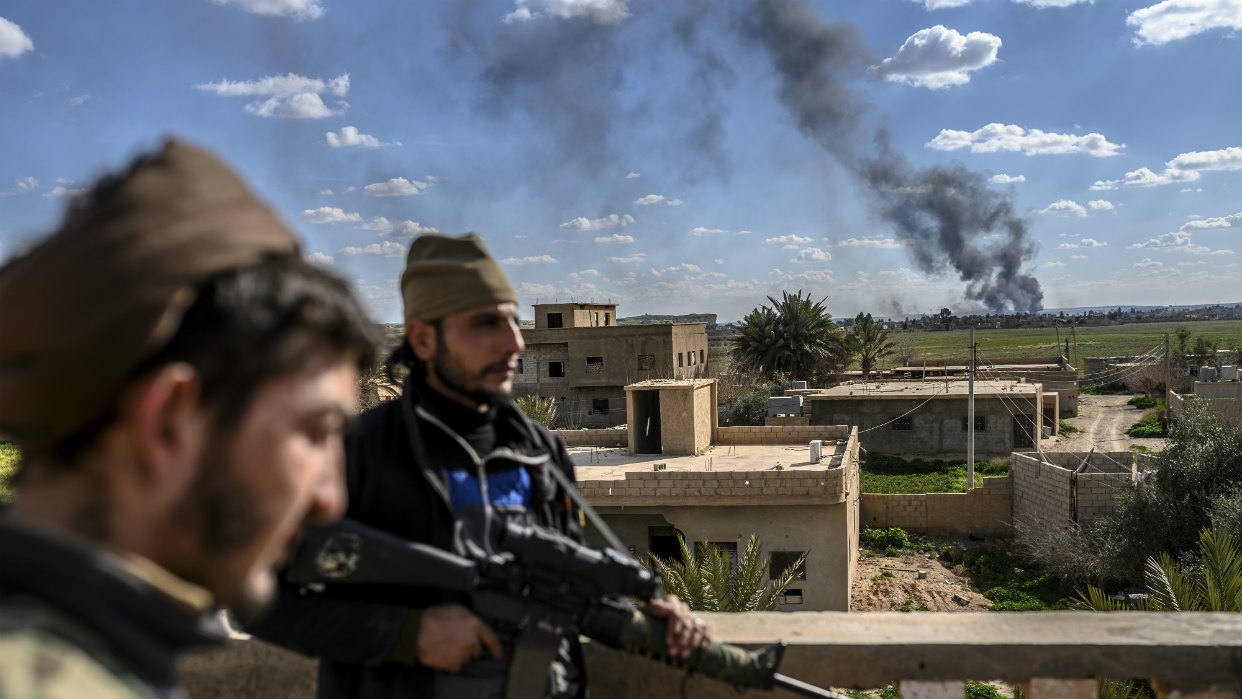
\includegraphics[width=300px]{EU_34908.jpg}%
\newline%
%
Los combatientes kurdos y árabes de las Fuerzas Democráticas Sirias (FDS) habían reanudado el viernes su ofensiva en la localidad de Baghuz, pero tuvieron que interrumpirla ya que miles de mujeres y niños, así como numerosos heridos abandonaron el sector los últimos días. Los últimos yihadistas están allí acorralados, destacó AFP.%
\newline%
%
Tras el atardecer en Baghuz, las FDS bajaron de un camión a numerosas mujeres heridas, en sus posiciones.%
\newline%
%
Muchas de ellas tuvieron que ser transportadas en camilla, en tanto médicos de la ONG estadounidense Free Burma Rangers atendían a las recién llegadas, envolviendo en una manta a una mujer cuya condición requería una atención inmediata.%
\newline%
%
Oleadas no finalizan%
\newline%
%
Detrás de ellas, una solemne procesión de hombres barbudos, custodiados por milicianos armados, avanzaba lentamente hacia las tropas de la coalición y los combatientes de las FDS, que intentan identificar a posibles yihadistas.%
\newline%
%
Las mujeres, de negro y con los ojos en lágrimas, se acercaban para observarlas y preguntaron a las FDS adónde iban a llevarlos.%
\newline%
%
Entre los evacuados había varios niños, entre ellos siete yazidíes, minoría que sufrió en particular los abusos de EI.%
\newline%
%
"Cada vez que creemos que se trata de la última oleada, hay nuevas salidas" del reducto yihadista, dijo un responsable de las FDS bajo condición del anonimato.%
\newline%
%
Desde el techo de un edificio en Baghuz, en donde están desplegados combatientes de las FDS, se veía el miércoles una columna de humo en el sector controlado por los yihadistas, que alcanza sólo a unas casas linderas a un campamento improvisado.%
\newline%
%
Los aviones de la coalición internacional están permanentemente sobrevolando el sector, pero se abstienen de atacar.%
\newline%
%
Entre las posiciones de las FDS y el campamento se ven una decena de carcasas de coches carbonizadas. En el campamento se ve hombres corriendo entre las carpas.%
\newline%
%
Los que salieron el martes de Baghuz, en su mayoría venidos de Francia, Bélgica o Finlandia, aseguran que aún habría varias miles de personas en el bastión yihadista.%
\newline%
%
'Traumatismo'En los llanos cerca de Baghuz, un océano de mujeres en niqab negro formaban fila el martes para ser registradas.Luego de ser registradas, muchas de ellas se instalan en el piso con sus bebes, en medio de botellas de agua, pan y pañales que les fueron distribuidos.También hay hombres, recostados sobre camillas o en equilibrio con muletas."Aun hay mucha gente", dice una belga de 24 años, que creció en Francia y que se presenta como Safia.Su marido, un francés, sigue en el sector de los yihadistas. Sólo quiere "descansar y pensar" dice la mujer que salió "de un traumatismo".En 2014 los yihadistas del grupo Estado Islámico lanzaron una ofensiva relámpago que les permitió autoproclamar en junio de ese año un "califato" en Siria e Irak.Miles de extranjeros, entre ellos europeos, se unieron al grupo yihadista que desde hace dos años pierde terreno por las múltiples ofensivas.Más de 57.000 personas, principalmente familiares de yihadistas, dejaron el último bastión desde principios de diciembre, según el Observatorio Sirio de Derechos Humanos (OSDH). Entre ellas, más de 6.000 yihadistas fueron detenidos, según esta fuente.'Necesidades urgentes'Los civiles evacuados, entre ellos las esposas e hijos de los yihadistas, son trasladados hacia campamentos de desplazados en el noreste sirio. Principalmente el de Al Hol, en donde decenas de miles de personas viven en condiciones difíciles, denunciadas por las ONG."La necesidad más urgente sigue siendo un techo", pero también asistencia médica, "física y psicológica", "en particular para los grupos vulnerables, como las mujeres embarazadas, los niños y los ancianos", subrayaba el lunes la Oficina de la ONU para la Coordinación de Asuntos Humanitarios (OCHA) en Siria."El seguimiento de numerosos casos de niños no acompañados y separados (de sus familias) sigue siendo una prioridad", agregaba la agencia.Si ISIS pierde su último bastión en Baghuz sería el fin del "califato".Pero el grupo ya comenzó a transformarse en organización clandestina. Aún hay combatientes dispersos en el vasto desierto del centro sirio.La batalla contra ISIS es hoy el principal frente de la guerra en Siria que dejó desde 2011 más de 360.000 muertos.%
\newline%
%
\end{document}